%!TEX root = ../main.tex

%%%%%%%%%%%%%%%%%%%%%%%%%%%%%%%
%%%%%%%%%%%%%%%%%%%%%%%%%%%%%%%
\chapter{Revitalization of the OLTC} % for Modern Grid Requirements}
\label{chap:intro}

\begin{textblock*}{.7\textwidth}(70mm-\offset,25mm-\offset)%(70mm,25mm)
    \begin{fquote}[Albert Einstein]
        % All models are wrong, but some are useful.
        Two things are infinite: the universe and human stupidity; and I'm not sure about the universe.
    \end{fquote}
\end{textblock*}

Some blibla as introduction. \autocite{machowski_2020}

\section{Research Interests}
\label{sec:research-interests}

Here are gaps and possible extension of knowledge.

Here are the research objectives and questions.

\commenting{
    \begin{itemize}[nosep]
        \item Influence of OLTC control on possible operational uses: Short-term voltage stability, long-term voltage stability; 
        \item Can a increased dynamic regulation help machine recovery?
        \item Does the increased tap ratio gradient harm transient stability of machines?
        Does it help or harm CCT of machines or machine groups?
        \item Transformers act as big low-pass filters: Can this behavior be beneficial as well for the interactions of inverters in the grid on AC side (in the sense of Harmonic Stability)? \quelle
    \end{itemize}
}

\begin{tcolorbox}[float, colback=ees_blue!5!white,colframe=ees_blue, toptitle=1mm, bottomtitle=1mm, left=2mm, right=2.5mm, top=2mm, bottom=2mm, title={\textbf{Research Question of this Thesis}}]
    How do different control types and characteristics of Tap Changing transformers influence the voltage stability of the given system?
\end{tcolorbox}

\sidenote{Influence of FSM on Voltage Stability}
Therefore following questions/steps can be imagined as supportive:
\begin{enumerate}
    \item How can Voltage stability of a system be classified and be looked at? Which indices, measurements, etc.
    \item Which transformer model has to be considered to show influences?
    \item Which systems are useful to consider in showing effects? Which circumstances lead to a stability support, which to a decrease? Where can limits be drawn?
\end{enumerate}

Additionally during the process of the thesis, the following question came up as an extension.
Is is the second interest of this thesis, and shall be more focused in the later part.
Therefore some assessments in the \autoref{chap:case-study} are conducted.

\begin{tcolorbox}[float, colback=ees_green!5!white,colframe=ees_green, toptitle=1mm, bottomtitle=1mm, left=2mm, right=2.5mm, top=2mm, bottom=2mm, title={\textbf{Additional Question of this Thesis}}]
    Can the already existing Tap Changer Control of the \acf{FSM} be improved towards a more operation oriented control?
\end{tcolorbox}

\sidenote{FSM Control Advancement? Operational Oriantation}
This question has following thoughs, concerning the different characteristics and dynamics of the \acs{FSM}:
\begin{enumerate}
    \item How do the different time constants of \acs{OLTC} and \acs{FSM} influence different stybility aspects in the system?
    \item Can the \acs{FSM} be used as a \glqq damping element\grqq~in the system?
    \item Does this possible different behavior of the \acs{FSM} lead to different operating strategy?
    \item What are thoughts on realizing such a strategy with different approaches on the \acs{FSM} controller?
\end{enumerate}

\section{Readers Guide}

The afore stated research interests in combination with the yet not sufficient framework to use make demands on the structure of this work. 
Therefore it seems not sufficient trying to apply a completely standard sequence of chapter like \glqq Introduction - Fundamentals - Methods - Results - Discussion\grqq.
Instead, the following structure is chosen to fulfill the research interests and to give a clear and understandable overview of the work.
This leads to the following structure for the thesis: 
\begin{itemize}
    \item \textbf{\hyperref[chap:fundamentals]{Chapter 2: Fundamentals},}\\
    is illustrating and recalling fundamentals for modeling, stability assessments, and discussions;
    \item \textbf{\hyperref[chap:methodical-modeling]{Chapter 3: Methodical Modeling},}\\
    describes the process of modeling in the tool \textit{diffpssi}, and the implementation of voltage stability indices;
    \item \textbf{\hyperref[chap:verification]{Chapter 4: Verification Setup and Result},}\\
    is showing the verification of the implemented models and tools with the help of common and simple test systems;
    \item \textbf{\hyperref[chap:case-study]{Chapter 5: Case Study},}\\
    is looking at the novel control methods from different perspectives and applications; 
    \item \textbf{\hyperref[chap:discussion]{Chapter 6: Discussion},}\\
    discusses the FSM control strategies, considering the fundamentals, verification, and case study results;
    \item \textbf{\hyperref[chap:summary]{Chapter 7: Summary},}\\
    is summarizing with regards to the research questions, and looking towards research potential and future developments. 
\end{itemize}

When reading this thesis, one might consider its motivation and its prior knowledge for allocating attention to the different chapters.
For someone interested in the strategic development of the \acs{FSM} or \acsp{OLTC} in general, the introduction with its research interests (\autoref{sec:research-interests}) are most important. 
Combined with the Summary and Outlook (\autoref{chap:summary}), the containts of the thesis, answers to the research questions and some perspectives are included.
For this level basic knowledge in power system stability and the electrical energy grid is sufficient.
When one is also interested in the explanations and thoughts why the answers to the research questions are as they are, the chapter \autoref{chap:discussion} is additionally recommended. Eventaully, the chapter \autoref{chap:fundamentals} is giving a few basics for an eased understanding of discussion itself.
The third level would be a demonstration of practical applications in the case studies (\autoref{chap:case-study}).
Lastly, if one wants to further improve or develop the tool {\itshape diffpssi} or the control strategies in particular, the chapters \autoref{chap:methodical-modeling} and \autoref{chap:verification} are recommended.
Additionally the referenced literature and the \autoref{app:power-system-modeling} are giving valuable insights and information.

% % \vspace*{6pt}

% \begin{tcolorbox}[colback=ees_blue!5!white,colframe=ees_blue, left=2mm, right=2.5mm, top=2mm, bottom=2mm]
%     \textbf{\hyperref[chap:fundamentals]{Chapter 2}}: Fundamentals
% \end{tcolorbox}

% \sidenote{Laying out the Edge of Development}
% The Fundamentals part of the thesis shall introduce the reader to the state-of-the-art connection points in standard literature and newer publications. 
% It is not starting at basic concepts in electrical or control engineering theory, but is trying to summarize the most important basics. 
% The reader shall be able to quickly adapt and think through the later applied methods, gathered results, and discussions. 
% It is further into stability topics, mathematical representation of transformers in simulations, and some informations about current applied control standards in the field of \acs{OLTC} transformers.
% \vspace*{6pt} 

% \begin{tcolorbox}[colback=ees_blue!5!white,colframe=ees_blue, left=2mm, right=2.5mm, top=2mm, bottom=2mm]
%     \textbf{\hyperref[chap:methodical-modeling]{Chapter 3}}: Methodical Modeling
% \end{tcolorbox}

% \sidenote{How are Things Done?}
% This chapter describes the advancements of the tool {\itshape diffpssi}, mainly the modeling of a ratio enabling $\Pi$-model for transformers and control circuits for their regulation. 
% Further it applies usable indices for a voltage stability assessment in the simulation environment. 
% Further, an assessment of the theoretical load-voltage boundaries is considered as well. 
% The chapter is mainly focussing on the implementation and interfaces towards the rest of the software.
% \vspace*{6pt} 

% \begin{tcolorbox}[colback=ees_blue!5!white,colframe=ees_blue, left=2mm, right=2.5mm, top=2mm, bottom=2mm]
%     \textbf{\hyperref[chap:verification]{Chapter 4}}: Verification Setup and Results
% \end{tcolorbox}

% \sidenote{Is the Tool Working?\\How Accurate is it?}
% The verification of the implemented models and tools is crucial for further studies and their validity. 
% Obtaining, discussing, and knowing the limits and boundaries of the tool is the main goal of this chapter. 
% Therefore the verification is done with the help of common and simple test systems, and the results are compared to a well known and widespread simulation tool {\itshape DIgSILENT PowerFactory} in the version 2023.
% \vspace*{6pt}

% \begin{tcolorbox}[colback=ees_blue!5!white,colframe=ees_blue, left=2mm, right=2.5mm, top=2mm, bottom=2mm]
%     \textbf{\hyperref[chap:case-study]{Chapter 5}}: Case study
% \end{tcolorbox}

% \sidenote{A Look from Different Perspectives}
% In the case study, some interesting found aspects are tried to pick up and to be further investigated. 
% The main goal is, with the background of both research questions, to show the influence of different control types and characteristics of Tap Changing transformers on the voltage stability of the given system. 
% The results are compared with the help of indices, introduced in the previous chapters, and theoretical boundaries.
% \vspace*{6pt}

% \begin{tcolorbox}[colback=ees_blue!5!white,colframe=ees_blue, left=2mm, right=2.5mm, top=2mm, bottom=2mm]
%     \textbf{\hyperref[chap:discussion]{Chapter 6}}: Discussion of the Results
% \end{tcolorbox}

% \sidenote{What Did we Learn? How can We make Use?}
% Discussing the results from the previous case studies combined with the verifacation and validation results, and the technological fundamentals rounds up the evaluation of the novel control strategies in a system perspective. 
% It shall demonstrate well suited applications, as well as current and possibly sustaining limits of the \acs{FSM}.
% \vspace*{6pt}    

% \begin{tcolorbox}[colback=ees_blue!5!white,colframe=ees_blue, left=2mm, right=2.5mm, top=2mm, bottom=2mm]
%     \textbf{\hyperref[chap:summary]{Chapter 7}}: Summary and Outlook
% \end{tcolorbox}

% The last chapter is summarizing the thesis with regards to the first initiated research questions. 
% In addition, an outlook is given in the sense of possible further research and development steps, or perspectives for application of the covered topics in this work.

%%%%%%%%%%%%%%%%%%%%%%%%%%%%%%%
%%%%%%%%%%%%%%%%%%%%%%%%%%%%%%%
\chapter{Fundamentals}
\label{chap:fundamentals}

\begin{textblock*}{.7\textwidth}(70mm-\offset,25mm-\offset)
    \begin{fquote}[Frank Zappa]
        So many books, so little time.
    \end{fquote}
\end{textblock*}

Following chapter shall introduce the basics for implementing an \acs{OLTC} equipped transformer into a existing \acs{PSS} framework.
This is considering the already existing surrounding, more detailed the electric behavior of the transformer itself and some control engineering theory for the corrosponding \acs{OLTC}. 
Thus its main goal is increasing voltage stability \autocite{machowski_2020}, main indices and assessment methods are considered as well.

\commenting{
    % Transformer $\Pi$-Model:
    % \begin{itemize}[nosep]
    %     \item Deviation from 'normal' circuit
    %     \item Placing the impedance elements on the LV side vs. HV side
    %     \item Getting into a single line $\Pi$-model
    %     \item Introducing the tapping factor $\vartheta$; if phase shifting it is getting complex -> how to consider this
    %     \item Different Y-Bus matrices if LV or HV side is considered
    %     \item Per-unit problems with the transformer characteristics
    %     \item Short overview of Open-Source power system simulation packages
    % \end{itemize}
    Voltage stability:
    \begin{itemize}[nosep]
        \item Definitions, classifications, conditions
        \item PV-curves / QV-curves
        \item Derivation of Indices: Practical application
    \end{itemize}
    Control engineering:
    \begin{itemize}[nosep]
        \item State-of-the-art control mechanisms for OLTCs
        \item Chaos theory controllers
    \end{itemize}
}

%%%%%%%%%%%%%%%%%%%%%%%%%%%%%%%
\section{Voltage Stability Basics}
\label{sec:voltage-stability}

% \subsection{Voltage Stability Definitions, Classifications, and Conditions}
A Practical introduction to voltage stability assessment, methods and indices is given in the standard and extending literature of \textcite{rueda-torres_2024,danish_2015,cutsem_1998}.

\commenting{
    Interesting to note/implement here: Basic classification, definitions, and the nature or conditions of voltage stability. Such as
    \begin{itemize}[nosep]
        \item Short term vs. long term
        \item Static vs. dynamic
        \item Transmission driven vs. load driven vs. generation driven; stability/instability, and/or contributions 
        \item Influence OLTC: Restoring voltage level, but not adding reactive capacities; hence adding risk of voltage collapses
        \item Load vs. transmission aspects
        \item Example mechanism: \textbf{Collapse effect of the nordic test system} \autocite{vancutsem_2020,cutsem_1998}
    \end{itemize}
}
        
\begin{table}
    \centering
    \caption[Voltage instability types and different time frames]{Voltage instability types and different time frames with examples; after \quelle}
    \small
    \renewcommand\tabularxcolumn[1]{m{#1}}
    \vspace*{12pt}
    \begin{tabularx}{\textwidth}{llXX}
        \toprule
        \textbf{No} & \textbf{Type} & \textbf{Cause of incident} & \textbf{Time frames} \\
        \toprule
        1 & Long-term & Slowly use up of reactive reserves and no outage & Several minutes to several hours \\
        2 & Classical & Key outage leads to reactive power shortage & One to five minutes \\
        3 & Short-term & Induction motor stalling leads to reactive power shortage & Five to fifteen seconds \\
        \bottomrule
    \end{tabularx}
\end{table}

        
\subsection{Analytical Stability Calculation of Simple Static Power Systems}
\label{sec:analytical-voltage-stability}

\subsection{Stability Limits of Complexer Systems: Continuation Power Flow}
\label{sec:continuation-power-flow}

\subsection{Stability Indices for Time Series Calculation}
\label{sec:stability-indices}

\sidenote{Basic idea and references}
The idea behind stability indices is monitoring the current voltage stability state of the power system in relation to the critical point.
This applies not only to static load flow cases, but for time series calculations of short circuits, load shedding or other disturbances.
Therefore the dynamic contribution can be included as well. \quelle

Reviewing possible indices, either for online resp. real time monitoring or for subsequent analysis after a simulation, is out of the scope of this thesis.
\textcite{danish_2015} has already included an extensive review in his work, with reference to \textcite{doigcardet_2010}, which is focussing on indices in interest for this thesis in particular. 
\commenting{Jacobian Matrix based interesting, because of the possible observability in \textit{diffpssi}.}

\sidenote{The basics of the Jacobian Matrix}
One easy idea for obtaining a stable operation is looking at the Jacobian Matrix. 
Although it is mainly used in load flow calculations, it is possible to derive statements about the voltage stability as well.
This can be realized through the relation of real power $P$, reactive power $Q$, voltage angle $\delta$, and the voltage resp. voltage gradients $\Delta V$. 
If the Jacobian Matrix is getting singular, the System will not remain in a stable operation.
Singularity of matrices is checked by following two hypothesis tests:
\begin{align}
    &\det(\mab{J})=0 \label{eq:jacobian-det} \\[12pt]
    &J \times J^{-1} \uparrow \label{eq:jacobian-rank}
\end{align}
The Jacobian Matrix is defined as:
% \sidenote(5.2cm){Jacobian Matrix}
\begin{align}
    \mab{J}=
    \begin{bmatrix}
        \Delta \mab{P} \\
        \Delta \mab{Q}
    \end{bmatrix}&=
    \begin{bNiceArray}{c|c}
        \mab{H} & \mab{M'} \\ \hline
        \mab{N} & \mab{K'}
    \end{bNiceArray} \cdot
    \begin{bmatrix}
        \Delta \delta \\
        \Delta V/V
    \end{bmatrix} \notag \\[12pt]
    \begin{bmatrix}
        \Delta P_1 \\
        \vdots \\
        \Delta P_n \\ \hline
        \Delta Q_1 \\
        \vdots \\
        \Delta Q_n
    \end{bmatrix}&=
    \begin{bNiceArray}{ccc|ccc}
        \frac{\partial P_1}{\partial \delta_1} & \hdots & \frac{\partial P_1}{\partial \delta_n} & V_1\frac{\partial P_1}{\partial V_1} & \hdots & V_n\frac{\partial P_1}{\partial V_n} \\
        \vdots & \ddots & \vdots & \vdots & \ddots & \vdots \\
        \frac{\partial P_n}{\partial \delta_1} & \hdots & \frac{\partial P_n}{\partial \delta_n} & V_1\frac{\partial P_n}{\partial V_1} & \hdots & V_n\frac{\partial P_n}{\partial V_n} \\ \hline
        \frac{\partial Q_1}{\partial \delta_1} & \hdots & \frac{\partial Q_1}{\partial \delta_n} & V_1\frac{\partial Q_1}{\partial V_1} & \hdots & V_n\frac{\partial Q_1}{\partial V_n} \\
        \vdots & \ddots & \vdots & \vdots & \ddots & \vdots \\
        \frac{\partial Q_n}{\partial \delta_1} & \hdots & \frac{\partial Q_n}{\partial \delta_n} & V_1\frac{\partial Q_n}{\partial V_1} & \hdots & V_n\frac{\partial Q_n}{\partial V_n} \\
    \end{bNiceArray} \cdot
    \begin{bmatrix}
        \Delta \delta_1 \\
        \vdots \\
        \Delta \delta_n \\ \hline
        \Delta V_1/V_1 \\
        \vdots \\
        \Delta V_n/V_n
    \end{bmatrix}
\end{align}

Although this method seems easy to implement, there are some numerical problems realted to that.
Checking if a Matrix is singular with numerical methods, can only be realised as a probablilty expression. 
A result could be, that the determinant of the matrix is below a certain threshold. 
The algorithm would propose, that the matrix is probabilistic singular. \quelle

\sidenote{Indices adressing numerical problems}
This problem leads to the necessity of applying other methods or indices for stability assessment. 
Further, the relation of the system state to the critical voltage collapse point is highly nonlinear in the Jacobian Matrix. 
This problem is adressed by the indices in various ways, leading to a more or less linearized relation. 
\quelle \textcite{danish_2015} is proposing a few other indices, that are based on the Jacobian Matrix, and shows comparitive characteristics between Jacobian Matrix and system variable based voltage stability indices. 
These Jacobian Matrix based indices are listed and further described in \autoref{app:jacobian-voltage-indices}, while the comparative characteristics are described in \autoref{app:jacobian-vs-system-indices}. 
The aforeside mentioned work of \textcite{doigcardet_2010} is focussing on these indices in particular.

For this thesis, the indices in \autoref{tab:considered-indices} are chosen on the basis of the work of \textcite{danish_2015} and \textcite{doigcardet_2010}. 
They will be implemented in the Python framework in \autoref{sec:application-voltage-stability}, and used for with the theoretical calculated limits of \autoref{sec:analytical-voltage-stability} and \autoref{sec:continuation-power-flow}.

\begin{table}[htb!]
    \centering
    \caption[Voltage stability indices for the assessment in this thesis]{Voltage stability indices for the assessment of the power system stability in this thesis; after \quelle}
    \label{tab:considered-indices}
    \vspace{12pt}
    \begin{tabularx}{\textwidth}{llX}
        \toprule
        \textbf{Index} & \textbf{Basis} & \textbf{Description} \\
        \toprule
        VCPI & Jacobian Matrix & The index is based on the Jacobian Matrix, and is showing the proximity of the current system state to the critical voltage collapse point. \\
        VSI & System Variables & The index is based on the system variables, and is showing the proximity of the current system state to the critical voltage collapse point. \\
        \bottomrule
    \end{tabularx}
\end{table}

\section{Voltage Angle Stability of Machines}

\commenting{
    Just short and briefly Describe
    \begin{itemize}[nosep]
        \item What is Voltage Angle Stability?
        \item Why relevant to this thesis?
        \item How to evaluate: EAC and CCT of a generator
        \item Maybe something like a max. utilization of max power angle?
    \end{itemize}
}

%%%%%%%%%%%%%%%%%%%%%%%%%%%%%%%
\section{Power System Modeling}

The simulation of power systems is a crucial tool, not only for stability studies, but for evaluating extensions or modifications in the planning process, the development of Assistance systems for operational management, and many other applications. \quelle 
Due to the complexity of the systems, simulations are often simplified. 
Not only with model constraints, bus as well in the way of calculations. 
Mainly seperating between \acf{EMT} and \acf{RMS} simulations, the latter is used in this thesis. 
The \autoref{app:power-system-modeling} is giving more details, literature, and summarizing the processes behind the used tool \textit{diffpssi}, if the reader is further interested in the topic.

\subsection{Transformer Electric Model and Behavior}
\label{sec:trafo-model}

% \begin{figure}[htb!]
%     \centering
%     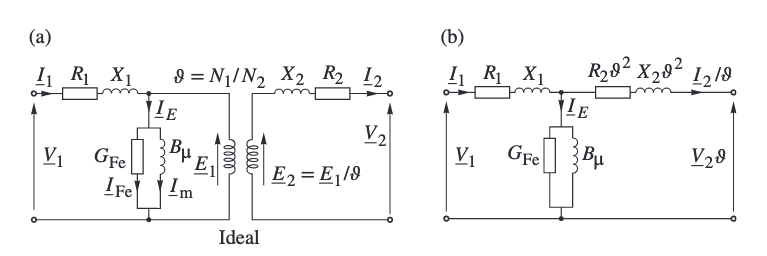
\includegraphics[width=.8\textwidth]{fundamentals/trafo_model_deviation.png}
%     \caption[Two-Winding Transformer Circuit in the Positive Sequence]{Two-Winding Transformer Circuit in the Positive Sequence; a) ideal representation with impedances on each \acs{HV} and \acs{LV} side and b) related impedances on the XX side; own figure after \autocite{machowski_2020}}
%     \label{fig:trafo-model-deviation}
% \end{figure}

% \sidenote{Basics}
Typical for \acs{RMS}-modeling is the usage of sequence components, especially the positive sequence for symmetrical grid operation and test cases. \quelle 
An equivalent circuit for the positive sequence is shown in \autoref{fig:trafo-model} part a), respectively reduced to the transformer ratio, the series impedances of the windings on the \acs{LV} and \acs{HV} side, and the shunt branch affected by iron and magnetization losses. \autocite{machowski_2020,kundur_2022,milano_2010}

The transformer ratio is typically noted as $\underline{\vartheta}$. 
Generally speaking it is the ratio between the number of windings of the secondary side to the primary side, as noted in \autoref{eq:trafo-ratio-easy}. 
With the typically used calculation unit \glqq per unit\grqq\footnote{means standardization to a reference value; further information on page \pageref{chap:symbols} and \textcite{machowski_2020}, Appendix A}, the ratio becomes one in the standard case. 
A transformer ratio, which is only shifting current angles with the shifting angle $\phi$, is represented through a complex number using the Euler Identity, as shown in \autoref{eq:trafo-ratio}.
\begin{align}
    \vartheta&=\frac{N_2}{N_1} \label{eq:trafo-ratio-easy} \\[6pt]
    \underline{\vartheta}&=\frac{N_2}{N_1} \cdot \exp(j \cdot \phi \cdot \frac{\pi}{180})\label{eq:trafo-ratio}
\end{align}

\begin{figure}% [htb!]
    \centering
    \captionsetup[subfigure]{justification=centering} 
    \begin{subfigure}[c]{.53\textwidth}
        \centering
        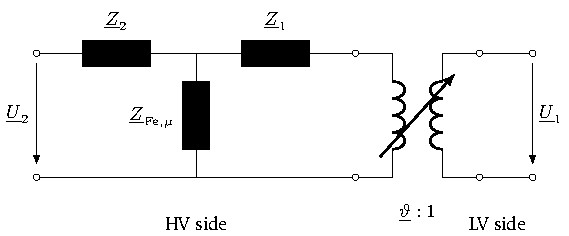
\includegraphics[width=\linewidth]{tikz_graphics/images/transformer_complete.pdf}
        \caption{}
    \end{subfigure}
    \begin{subfigure}[c]{.46\textwidth}
        \centering
        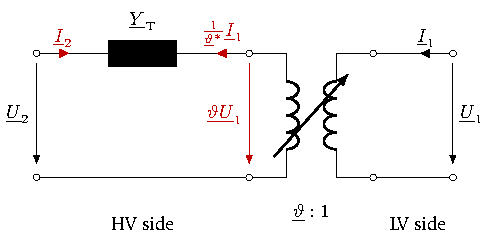
\includegraphics[width=\linewidth]{tikz_graphics/images/transformer_reduced.pdf}
        \caption{}
    \end{subfigure}
    % 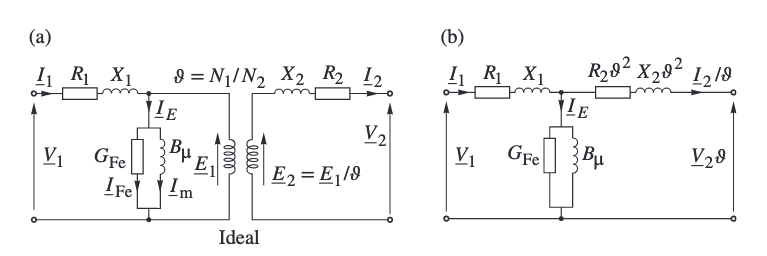
\includegraphics[width=.8\textwidth]{fundamentals/trafo_model_deviation.png}
    \caption[Two-Winding Transformer Circuit in the Positive Sequence]{Two-Winding Transformer Circuit in the Positive Sequence; a) ideal representation with impedances on the \acs{HV} side and b) simplifyied circit with only the series impedance related on the \acs{HV} side; own figure after \autocite{machowski_2020,kundur_2022,milano_2010}}
    \label{fig:trafo-model}
\end{figure}

\sidenote{Simplifications}
The first simplification is step is considering two assumptions. 
First, the iron and magnetization losses are neglectable. 
This can be illustrated with a short-circuit test of the transformer on the secondary side. 
During this test, one can obtain with the concept of a voltage devider, that
\begin{align}
    \underline{U}_\mathrm{Fe, \mu} \ll \underline{U}_\mathrm{T,rated}, \notag
\end{align}
meaning that the shunt branch impedance is much greater that the series impedance of the transformer. 
Secondly, it is assumed, that the on the primary side related impedance of the secondary side, is equal to the impedance on the primary side. 
This leads to a symmetrical circuit of the transformer and the positive sequence equivalent circuit simplifies to \autoref{fig:trafo-model} part b). 
Mathematically this is shortly expressable as \autoref{eq:related-impedances}, \autoref{eq:trafo-symmetrical}, and \autoref{eq:series-impedance}. \autocite{machowski_2020,kundur_2022,milano_2010}
\begin{align}
    \underline{Z}_1 &= R_1 + jX_1\text{;}\quad\underline{Z}_2 = R_2 \vartheta^2 + jX_2 \vartheta^2 \label{eq:related-impedances} \\
    \underline{Z}_1 &= \underline{Z}_2 \label{eq:trafo-symmetrical} \\
    \underline{Z}_\mathrm{T} &= \underline{Z}_1 + \underline{Z}_2 \label{eq:series-impedance}
\end{align}
The afore described simplification leads to only the necessity of considering the series impedance. 
Considering the afore mentioned normal ratio of $\vartheta=1$ in the per unit system, the Python framework \textit{diffpssi} has been using this model with only the series impedance and no variable ratio, meaning no shunt branches, before.

\sidenote{Introducing variable transformer ratios}
When one wants to look at variable transformer ratios, either with representing vector groups, or implementing \acfp{OLTC}, this model of only considering the series impedance has to be extended. 
Using shunt branches, the variable ratio behavior can be represented in a $\Pi$-model, as shown in \autoref{fig:pi-transformer}. \autocite{machowski_2020,kundur_2022,milano_2010}

\begin{figure}%[htb!]
    \centering
    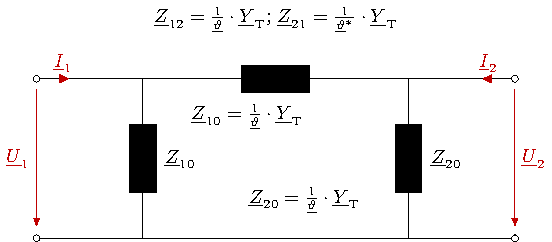
\includegraphics[width=.7\textwidth]{tikz_graphics/images/transformer_pi.pdf}
    \caption[$\Pi$-representative circuit of an idealized transformer with a tap changer]{$\Pi$-representative circuit of an idealized transformer with a tap changer; own figure after \autocite{milano_2010,burlakin_2024}}
    \label{fig:pi-transformer}
\end{figure}

Looking at the transformer as a black box two-port, with the index one being the \acs{LV} side, the index two being the \acs{HV} side, the admittance matrix for the variable ratio behavior can be expressed as in \autoref{eq:admittance-behavior}. 
The voltages and current are defined as in \autoref{fig:trafo-model} part b). 
With rearranging the equation, one can obtain the admittance matrix of the $\Pi$-model with to the \acs{HV} side related values as in \autoref{eq:admittance-matrix-pi}. \autocite{milano_2010,burlakin_2024}

\begin{align}
    \begin{bmatrix}
        {\color{ees_green}\underline{\vartheta}^*} \underline{I}_1 \\ \underline{I}_2
    \end{bmatrix}&= 
    \begin{bmatrix}
        \underline{Y}_\mathrm{T} & -\underline{Y}_\mathrm{T} \\
        -\underline{Y}_\mathrm{T} & \underline{Y}_\mathrm{T}
    \end{bmatrix} \cdot
    \begin{bmatrix}
        {\color{ees_green}\frac{1}{\underline{\vartheta}}}~\underline{U}_1 \\ \underline{U}_2
    \end{bmatrix} \label{eq:admittance-behavior} \\[12pt]
    \underline{\mab{Y}}_\mathrm{\Pi,T}&=\underline{Y}_\mathrm{T} \cdot
    \begin{bmatrix}
        \frac{1}{\underline{\vartheta}\underline{\vartheta}^*} & -\frac{1}{\underline{\vartheta}^*} \\
        -\frac{1}{\underline{\vartheta}} & 1
    \end{bmatrix} \label{eq:admittance-matrix-pi}
\end{align}

For calculation of the individual shunt branches, one can apply the standard representation of two-ports consistent of a linear $\Pi$-circuit:
\begin{align}
    \begin{bmatrix}
        \underline{I}_1 \\ \underline{I}_2
    \end{bmatrix}=
    \begin{bmatrix}
        \underline{Y}_{10} + \underline{Y}_{12}& -\underline{Y}_{12} \\
        -\underline{Y}_{21} & \underline{Y}_{20} + \underline{Y}_{21}
    \end{bmatrix} \cdot
    \begin{bmatrix}
        \underline{U}_1 \\ \underline{U}_2
    \end{bmatrix} \notag % \label{eq:shunt-calc}
\end{align}
When equating this with \autoref{eq:admittance-matrix-pi}, the shunt branches can be calculated respectivly giving the admittances written down as \autoref{eq:y-12}, \autoref{eq:y-10}, and \autoref{eq:y-20}, as they are noted in \autoref{fig:pi-transformer} as well. \autocite{milano_2010,burlakin_2024}
\begin{align}
    \underline{Y}_{12}&=\frac{1}{\underline{\vartheta} \cdot \underline{a}_\mathrm{T}^*} \cdot \underline{Y}_\mathrm{T}\text{, and} \notag \\[6pt]
    \underline{Y}_{21}&=\frac{1}{\underline{\vartheta} \cdot \underline{a}_\mathrm{T}} \cdot \underline{Y}_\mathrm{T} \label{eq:y-12} \\[12pt]
    \underline{Y}_{10}&=\frac{1}{\underline{\vartheta}} \cdot \bigg(\frac{1}{\underline{\vartheta}} - \frac{1}{\underline{a}_\mathrm{T}}\bigg) \cdot \underline{Y}_\mathrm{T} \label{eq:y-10} \\[12pt]
    \underline{Y}_{20}&=\bigg(1 - \frac{1}{\underline{\vartheta} \cdot \underline{a}_\mathrm{T}}\bigg) \cdot \underline{Y}_\mathrm{T} \label{eq:y-20}
\end{align}

% After MACHOWSKI:
% \begin{align}
%     \underline{\mab{Y}}_\mathrm{\Pi,T}&= 
%     \begin{bmatrix}
%         \underline{Y}_\mathrm{T} & -\underline{\vartheta}\underline{Y}_\mathrm{T} \\
%         \underline{\vartheta}^*\underline{Y}_\mathrm{T} & -\underline{\vartheta}^*\underline{\vartheta}\underline{Y}_\mathrm{T}
%     \end{bmatrix} \label{eq:admittance-oltc}
% \end{align}
% Another way of writing down the admittance matrix is shown in \autoref{eq:admittance-oltc-2}. It is considering, that the matrix can be split up in a symmetric, constant part, and a variable current injection part. The latter is not symmetrical and depends on the tap position of the transformer. Therefore in some simulation algorithms the static part is used in the admittance matrix, and the variable part is considered in the current injection vector. \autocite{machowski_2020}



\sidenote{Per unit system\\specialities}
Reactances and resistances are referred to the base voltage and apparent power of the operational unit, such as the transformer. 
The power system simulation uses its own base voltage and base apparent power, enabling the use of one single calculation domain. 
This is done to simplify the calculation and to make the results easily comparable to each other. 
Hence, the reffered values have to be transformed from the equipment based values to the simulation based values. 
The relation for the transformer admittance is defined as follows. 
Generally speaking, this thesis is using and reffering to the per unit based values, although it is not denoted in the index of the values.
\begin{align}
    \underline{Y}_\mathrm{T,~based}&=\underline{Y}_\mathrm{T} \cdot \frac{S_\mathrm{n}}{S_\mathrm{n,~sim}} \label{eq:y-t-based} \\[6pt]
    \underline{Z}_\mathrm{line,~based}&=\underline{Z}_\mathrm{line} \cdot \frac{S_\mathrm{n,~sim}}{V_\mathrm{n,~sim}^2} \label{eq:y-line-based}
\end{align}
Displayed like in \autoref{eq:y-t-based}, the characteristic of the operational unit is referred to the simulation base value. 
Here, the admittance of the transformer is multiplied with its own rated apparent power, then devided by the apparent power of the simulation system. 
Similar, the impedance of the lines are calculated via \autoref{eq:y-line-based}. 
This specialities are considered in the tap changer modeling, thus further information is given in \autocite{machowski_2020}, Appendix A.

\subsection{Further Considerations of a Transformer Model}
\label{sec:further-considerations}

\commenting{Describe here the asymetric and non-idealized transformer; phase shifting transformers; transformers, which can control logitudinal and transversal ratios; ...}

\sidenote{Ideal vs. asymmetric ratio}
\commenting{Just briefly desribe the influence of an asymetric vs. an ideal transformer. Why the difference and how the representation could work.}
\begin{figure}[htb!]
        \centering
        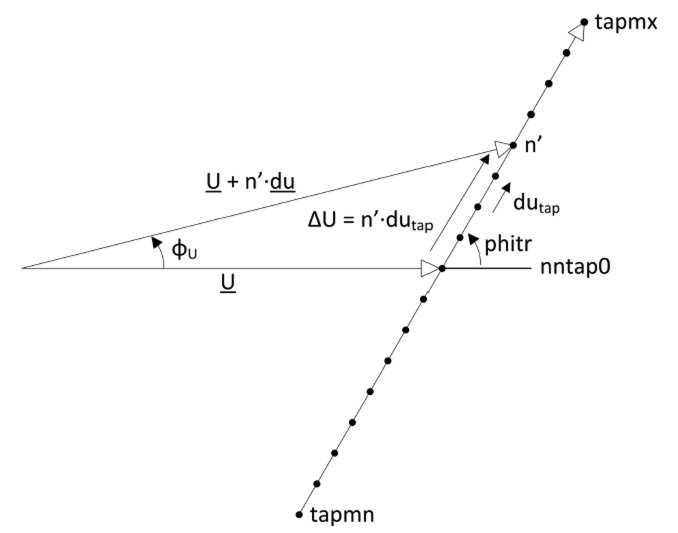
\includegraphics[width=.7\linewidth]{images/modeling/asymetric_ratio_vector.png}
        \caption[Illustration of the tap ratio vector for an ideal and an asymmetric transformer]{Illustration of the tap ratio vector for an ideal and an asymmetric transformer; from the \textcolor{ees_red}{\textbf{DIgSILENT Technical Reference Manual}} \dots \quelle}
        \label{fig:asymetric-ratio-vector}
\end{figure}

\subsection{Open-Source Power System Simulation tools}
    
\commenting{
    Some information about other open source python power system simulation tools, such as:
    \begin{itemize}[nosep]
        \item Pandapower,
        \item TOPS,
        \item ... .
    \end{itemize}
    Maybe relate to \href{https://github.com/ps-wiki/best-of-ps}{this GitHub Repo}, comparing different Open-Source Power System Simulation tools.
    Build up like a scan (see Georg's thesis).
}
        
%%%%%%%%%%%%%%%%%%%%%%%%%%%%%%%
\section{On-Load Tap Changer Controls}

\subsection{Commonly Used On-Load Tap Changer Control}

A few basics are in the interest, understanding differences between real world beahavior, or possible ways of building up a \acs{OLTC} transformer control. 
This control theory difference can be limiting as well for the results and objectives compared to the actual possible control in the field.

% \subsubsection{Typical presets are manually set}
\sidenote{Typical presets are manually set}
The target voltage is typically set from the control room of the grid operator, coming from pre-calculated load flow analysis. 
This can be set hours before, or even day-ahead with the estimated loads of the grid. 
This value is set locally for each operating unit subsequently. 
The control is then operating locally and without further involvement of the grid operator. \quelle

% \subsubsection{Discrete controllers are used in the field}
\sidenote{Discrete controllers are used in the field}
Typically the used controller in the field is a discrete controller, which can change tap positions under load within a time frame of around few seconds. 
Practical tap steps are around $2~\mathrm{\%}$ of the overall transforming ratio. 
The control is set up with a dead band, to avoid unnecessary tap changes. 
It is necessecary to note here, that this control and its mathematical caracteristics contains logical elements, blocks, and delays, which cannot be translated in a typical control theory transmission function. 
This leads to the missing possibility to easily obtain mathematical stability for the control of the overall considered power system. \quelle

\subsection{Advancement: Fast Switching Module and its Control}

\commenting{
    Describe the findings of Ilya:
    \begin{enumerate}[nosep]
        \item Approach and technological (short and not too detailed),
        \item Control proposal of Ilya,
        \item (Hardware) Development potential.
\end{enumerate}
}


%%%%%%%%%%%%%%%%%%%%%%%%%%%%%%%
\section{Summary in Short and Simple Terms}